\documentclass{standalone}
\usepackage{tikz}
\usepackage{pgfplots}

\begin{document}

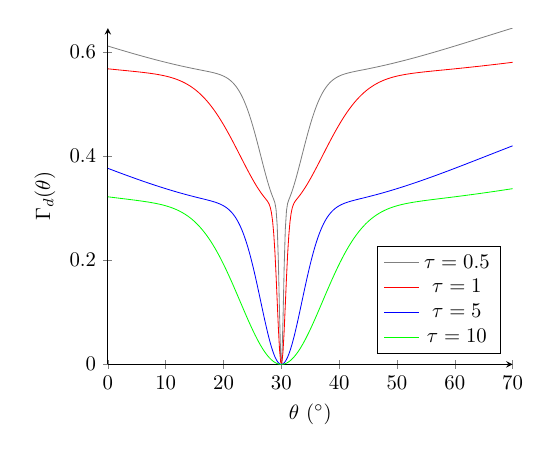
\begin{tikzpicture}[scale=0.75]
	\begin{axis}
		[
			axis lines = left,
			xlabel = $\theta\ (^\circ)$,
			ylabel = {$\Gamma_d(\theta)$},
			legend pos = south east,
		]
	\addplot
		[
			domain = 0:70,
			samples = 350,
			color = gray,
		]
	{1 - 1/2*(
		((6-0)/10)*exp(-((x-30)/(0.5*10^0))^2) +
		((6-1)/10)*exp(-((x-30)/(0.5*10^1))^2) +
		((6-2)/10)*exp(-((x-30)/(0.5*10^2))^2) +
		((6-3)/10)*exp(-((x-30)/(0.5*10^3))^2) +
		((6-4)/10)*exp(-((x-30)/(0.5*10^4))^2) )
		};
	\addlegendentry{$\tau = 0.5$}
	\addplot
		[
			domain = 0:70,
			samples = 350,
			color = red,
			]
	{1 - 1/2*(
		((6-0)/10)*exp(-((x-30)/(1*10^0))^2) +
		((6-1)/10)*exp(-((x-30)/(1*10^1))^2) +
		((6-2)/10)*exp(-((x-30)/(1*10^2))^2) +
		((6-3)/10)*exp(-((x-30)/(1*10^3))^2) +
		((6-4)/10)*exp(-((x-30)/(1*10^4))^2) )
	};
	\addlegendentry{$\tau = 1$}
	\addplot
		[
			domain = 0:70,
			samples = 350,
			color = blue,
			]
			{1 - 1/2*(
				((6-0)/10)*exp(-((x-30)/(5*10^0))^2) +
		((6-1)/10)*exp(-((x-30)/(5*10^1))^2) +
		((6-2)/10)*exp(-((x-30)/(5*10^2))^2) +
		((6-3)/10)*exp(-((x-30)/(5*10^3))^2) +
		((6-4)/10)*exp(-((x-30)/(5*10^4))^2) )
	};
	\addlegendentry{$\tau = 5$}
	\addplot
		[
			domain = 0:70,
			samples = 350,
			color = green,
		]
	{1 - 1/2*(
		((6-0)/10)*exp(-((x-30)/(10*10^0))^2) +
		((6-1)/10)*exp(-((x-30)/(10*10^1))^2) +
		((6-2)/10)*exp(-((x-30)/(10*10^2))^2) +
		((6-3)/10)*exp(-((x-30)/(10*10^3))^2) +
		((6-4)/10)*exp(-((x-30)/(10*10^4))^2) )
		};
		\addlegendentry{$\tau = 10$}
\end{axis}
\end{tikzpicture}
\end{document}